% PAKETE UND DOKUMENTKONFIGURATION
\documentclass[11pt, a4paper]{article}

% Encoding für Umlaute
\usepackage[utf8]{inputenc}

% Silbentrennung
\usepackage[ngerman]{babel}

% erweiterte Matheumgebungen
\usepackage{amsmath}

% zusätzliche mathematische Schriftarten
\usepackage{amsfonts}

% verschiedene mathematische Symbole
\usepackage{amssymb}

% Einheiten setzen z.B. \SI{10}{\kilo\gram\meter\per\second\squared}
% Fehler: \SI{10 +- 0,2e-4}{\metre}
\usepackage{siunitx}
\sisetup{
  output-decimal-marker={,},
  separate-uncertainty
}

% Randbreiten
\usepackage[left=3.5cm,right=3.5cm,top=3cm,bottom=3cm,twoside]{geometry}

% Bilder einfügen
\usepackage{graphicx}

% Verweise innerhalb des Dokuments
\usepackage{hyperref}
\hypersetup{
	colorlinks = true,
	allcolors = {black}
}

% bessere Tabellenlayouts
\usepackage{booktabs}

% Seitenlayout (Kopfzeile)
\usepackage{fancyhdr}

% Tiefe des Inhaltsverzeichnisses (Level: 1 sections, 2 subsections,
% 3 subsubsections)
\setcounter{tocdepth}{2}

% FANCYHDR SETUP
\pagestyle{fancy}
\fancyhead[EL,OR]{\thepage}
\fancyhead[ER]{\leftmark}
\fancyhead[OL]{\rightmark}

\renewcommand{\sectionmark}[1]{
\markboth{\thesubsection{} #1}{\thesection{} #1}
}
\renewcommand{\subsectionmark}[1]{
\markright{\thesubsection{} #1}
}


% DOKUMENTINFORMATIONEN
\title{P401 \\ Elektronische Übergänge in Atomen}

\author{Christopher Deutsch\footnote{christopher.deutsch@uni-bonn.de} \and Christian Bespin\footnote{christian.bespin@uni-bonn.de}}

\date{\today}

\begin{document}

\begin{titlepage}

\maketitle

% DURCHFÜHRUNGSDATUM UND ASSISTENT
\begin{center}
\begin{tabular}{l r}
Durchführung: & 17./18. November 2014 \\
Gruppe: & $\alpha$ 2 \\
Assistent: & ASSISTENT
\end{tabular}
\end{center}

% ZUSAMMENFASSUNG
\begin{abstract}
\noindent
% Text
\end{abstract}

\end{titlepage}

% INHALTSVERZEICHNIS
\tableofcontents
% Neue Seite nach TOC
\newpage

% INHALT VERSUCHSPROTOKOLL

\section{Grundlagen / Theorie}

\subsection{Zeeman-Effekt}

Der Zeeman-Effekt beschreibt die Aufspaltung entarteter Energien unter Einfluss eines äußeren Magnetfeldes.
In diesem Versuch wollen wir uns dabei auf den normalen Zeeman-Effekt beschränken; dieser gilt für Atome, deren Gesamtspin gleich $0$ ist und so nur Drehimpulse $\vec{L}$ zum Gesamtdrehimpuls $\vec{J}=\vec{L}+\vec{S}$ beitragen.

\subsubsection{Verhalten von Atomen in äußeren Feldern}

Aus der Lösung der Schrödingergleichung für ein Elektron im Coulombpotenzial eines Kerns folgt, dass es nur diskrete Energiewerte annehmen kann.
Diese werden über die so genannte Hauptquantenzahl $n$ bestimmt.
Zusätzlich dazu kann man weitere Quantenzahlen definieren, wir beschränken uns hier auf die Quantenzahl $l$ für den Drehimpuls und $s$ für den Spin.
Für $n$ und $l$ gilt $n=1, 2, 3 \dots$ und $l=0, 1, 2 \dots n-1$, wobei die Werte für $l$ häufig mit den Buchstaben s, p, d, f, g $\dots$ (ab f wie im Alphabet) identifiziert werden.
Da es nicht möglich ist, zwei Komponenten $L_i, L_j$ des Drehimpulses gleichzeitig zu bestimmen (folgt aus Kommutatorrelation), erhält man bei einer Messung von $|\vec{L}|$ und $L_z$, welche durchgeführt werden kann, eine weitere Quantenzahl $m_l$. Sie beschreibt im Vektormodell anschaulich die Projektion von $\vec{L}$ auf die $z$-Achse.
Dabei gilt:
\begin{align*}
|\vec{L}|&=\si{\planckbar}\sqrt{l(l+1)}\\
l_z&=\si{\planckbar}\mathrm{m}_l
\end{align*}

\begin{figure}
\centering
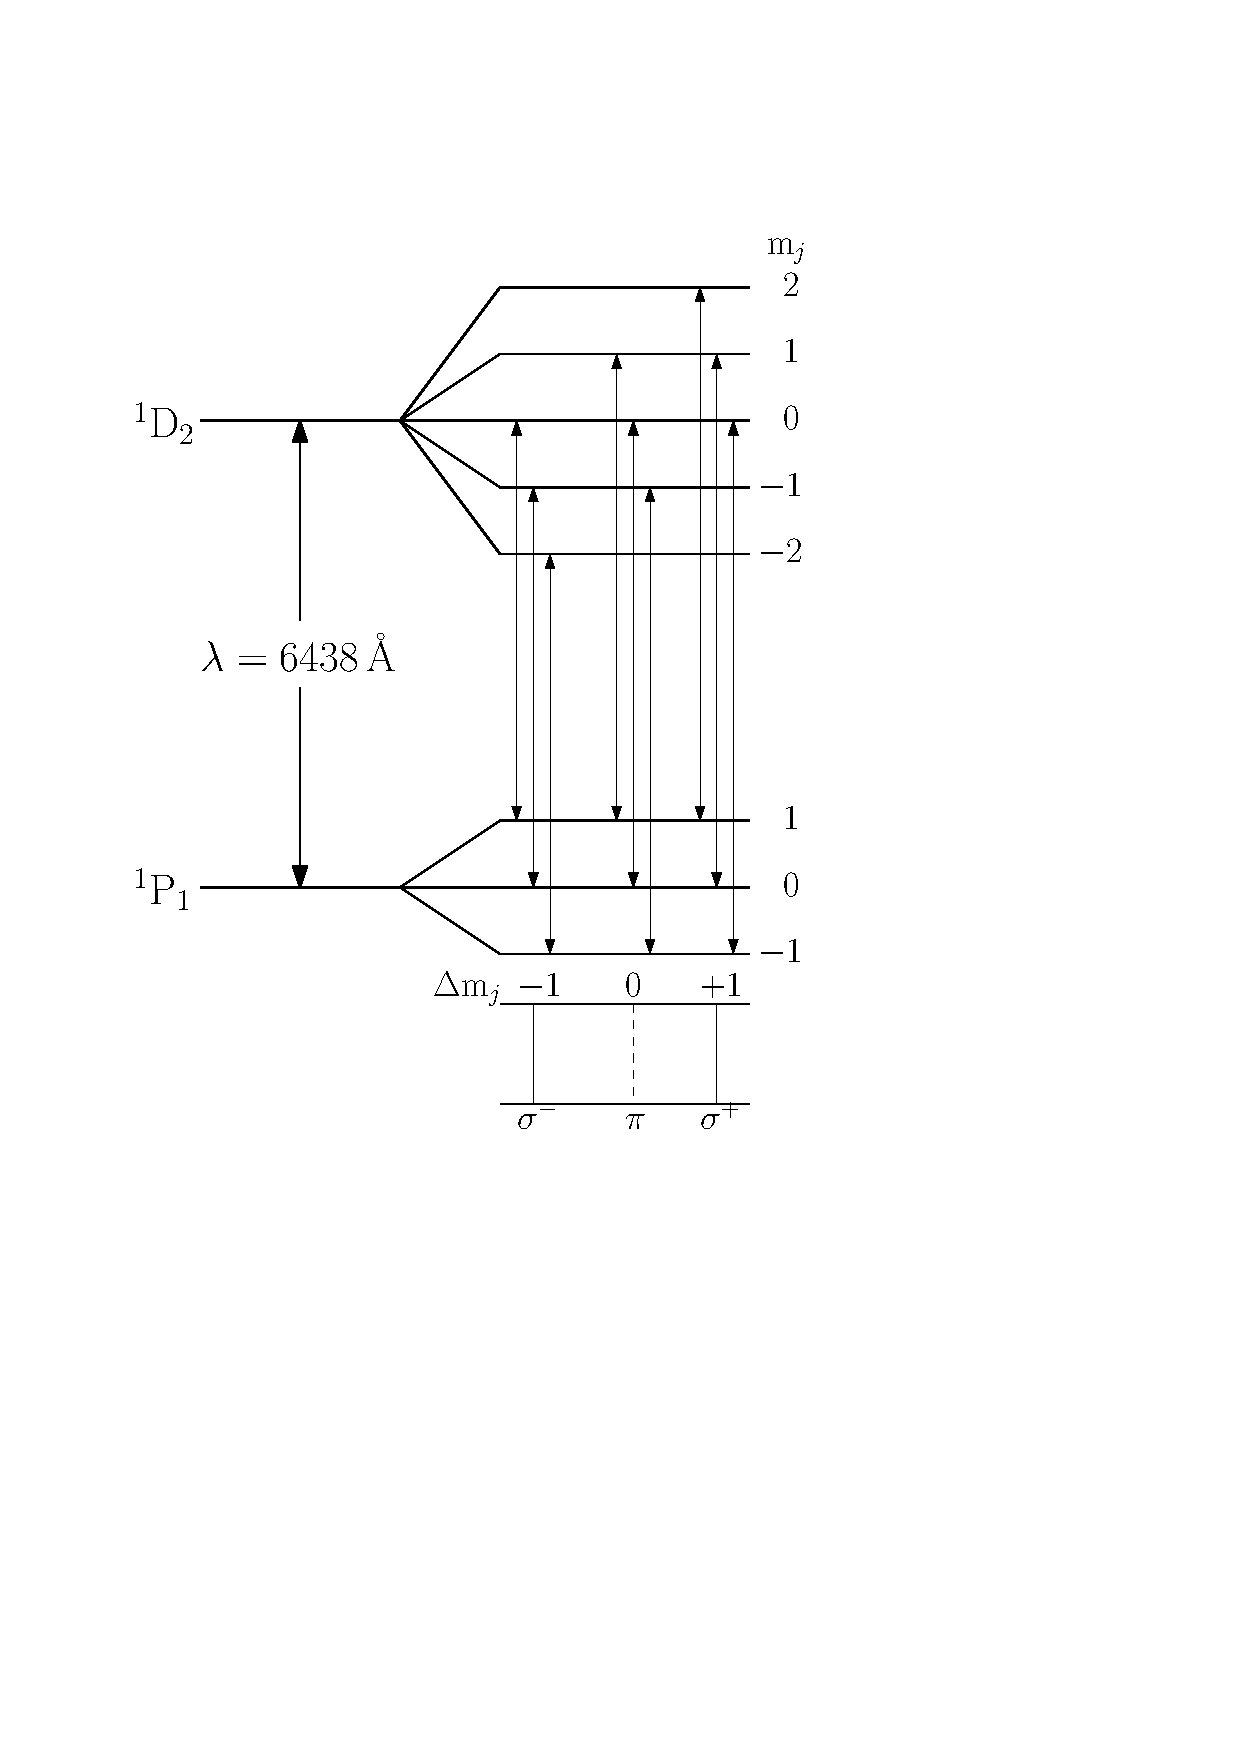
\includegraphics[width=0.4\textwidth]{./figures/termschema_cadmium.pdf}
\caption{Übergang von $^1$D$_2$ nach $^1$P$_1$ in der fünften Schale in Cadmium}
\label{fig:termschema_cadmium}
\end{figure}

\begin{itemize}
\item Zeeman Effekt
\item Niveauaufspaltung, Auswahlregeln und Übergänge von Cadmium
\end{itemize}

\subsubsection{Fabry-Pérot-Etalon}

\begin{itemize}
\item Funktionsprinzip
\item Auflösungsvermögen
\item Finesse
\end{itemize}

\subsubsection{Natürliche Linienbreite und Linienverbreiterung}

\subsubsection{$\frac{\lambda}{4}$-Platte}

\subsubsection{Hall-Sonde}

\subsection{Franck-Hertz-Versuch}

Der Franck-Hertz-Versuch wurde um 1914 von James Franck und Gustav Hertz \cite{demtroeder3} durchgeführt und demonstrierte die Wichtigkeit der Energiequantelung bei Stoßprozessen.
In dem Versuch wird eine mit Quecksilberdampf bei Unterdruck (ca. \SI{e-2}{\milli\bar}) gefüllte Elektronenröhre genutzt, bei der zwischen Kathode und Anode ein Gitter eingebaut ist, und die variable Beschleunigungsspannung $U$ zwischen Kathode und Gitter anliegt.
Zwischen diesem und der Anode wird eine konstante Gegenspannung $\Delta U$ angelegt.

\begin{figure}[h]
\centering
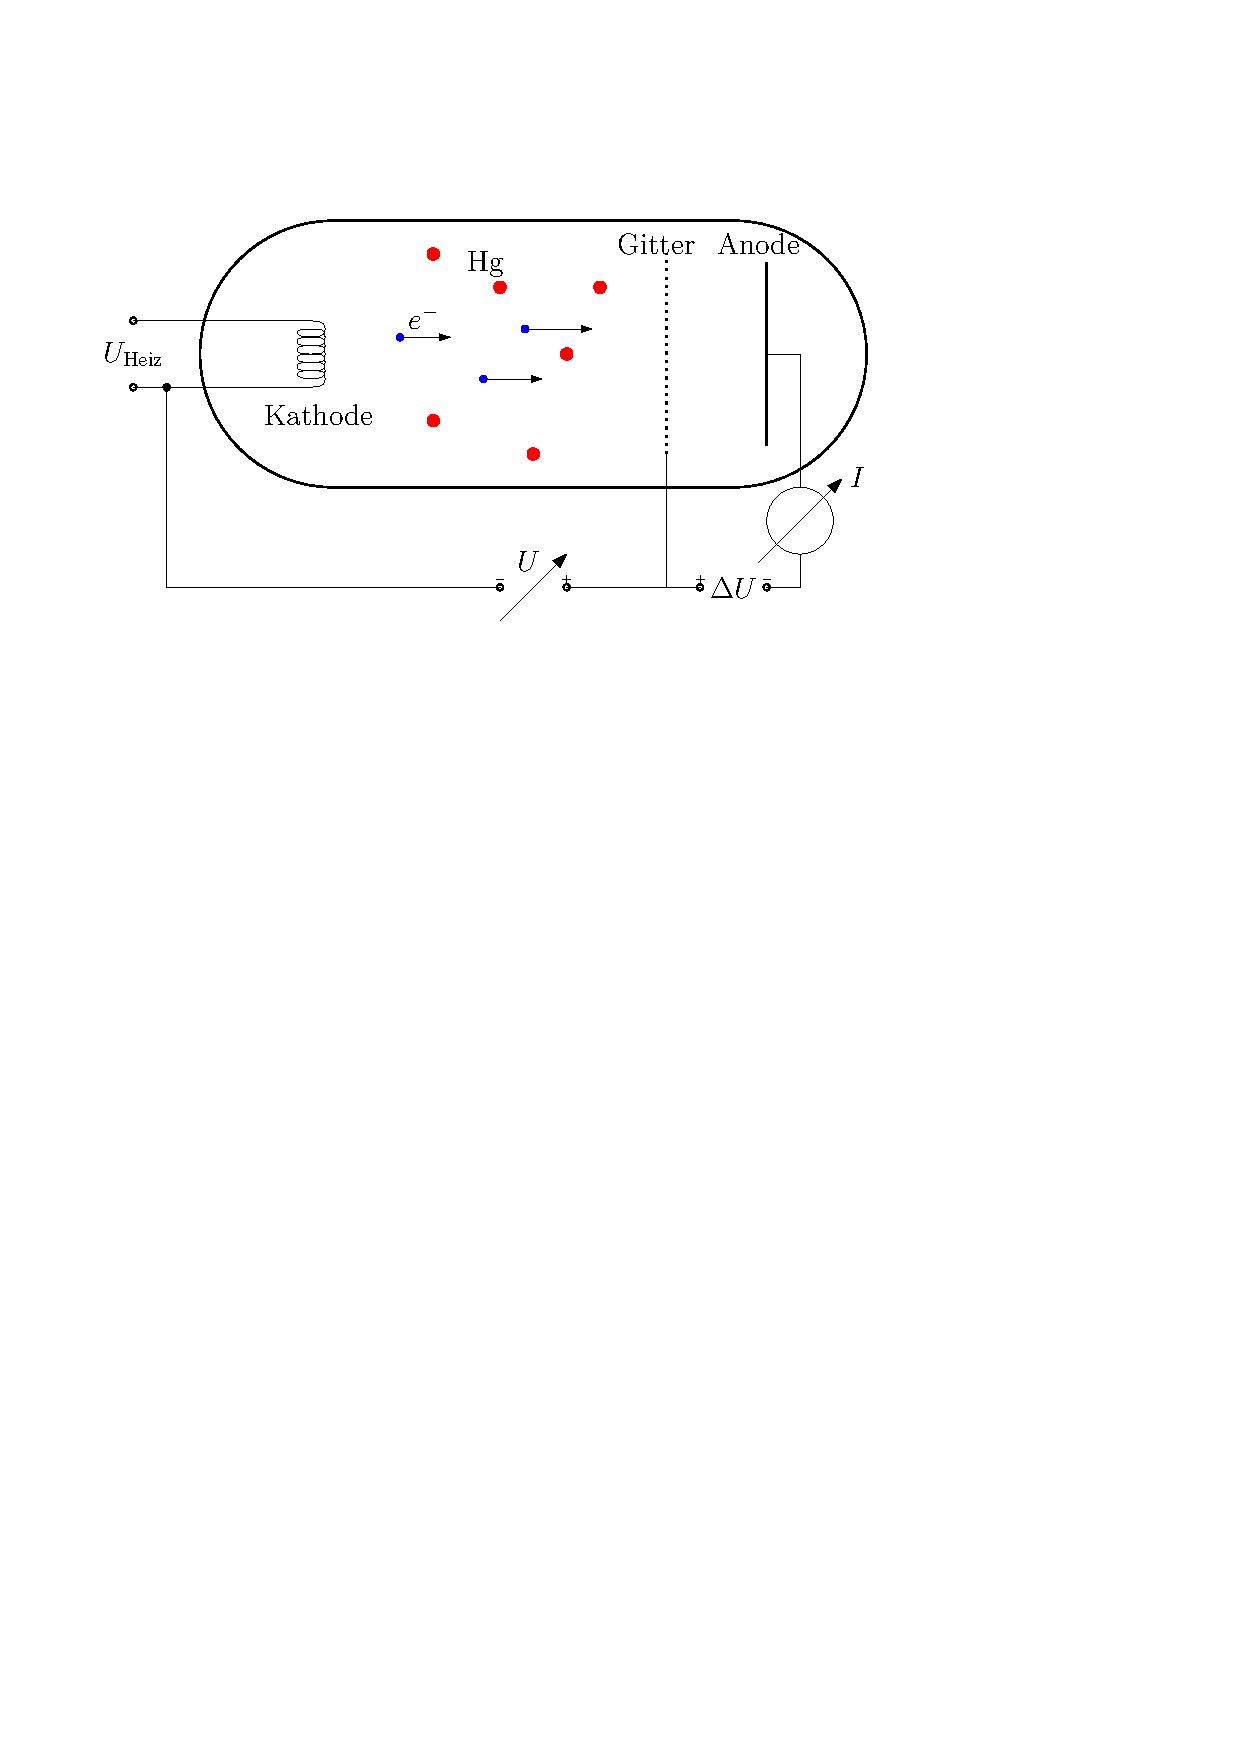
\includegraphics[width=0.7\textwidth]{./figures/franck-hertz_aufbau.pdf}
\caption{Aufbau des Franck-Hertz-Versuches}
\label{fig:franck-hertz_aufbau}
\end{figure}

Durch den glühlektrischen Effekt treten an der Kathode bei Anlegen einer hohen Spannung Elektronen aus.
Dies geschieht dadurch, dass die Elektronen im Draht durch die hohe Spannung angeregt werden und die (vom Material abhängige) Austrittsarbeit überwinden.
Die Stromdichte der aus einem Metall austretenden Elektronen wird beschrieben durch die \textbf{Richardson-Gleichung} \cite{np_richardson}:
\begin{align*}
j=AT^2\cdot \exp\left({-\dfrac{\omega}{\mathrm{k_B}T}}\right)
\end{align*}
Dabei ist $T$ die absolute Temperatur, $\mathrm{k_B}$ die Boltzmann-Konstante und $A$ und $\omega$ materialabhängige Konstanten.
Die so ausgetretenen Elektronen werden von dem äußeren anliegenden Feld durch die Beschleunigungsspannung zum Gitter hin beschleunigt und erreichen dabei die Energie $eU$.
Durch die zwischen Gitter und Anode anliegende Gegenspannung werden die Elektronen nach Passieren des Gitters abgebremst und nur solche mit Energien größer als $e\Delta U$ erreichen die Anode.
Der Aufbau bildet so ein Triodensystem.

\begin{figure}[h]
\centering
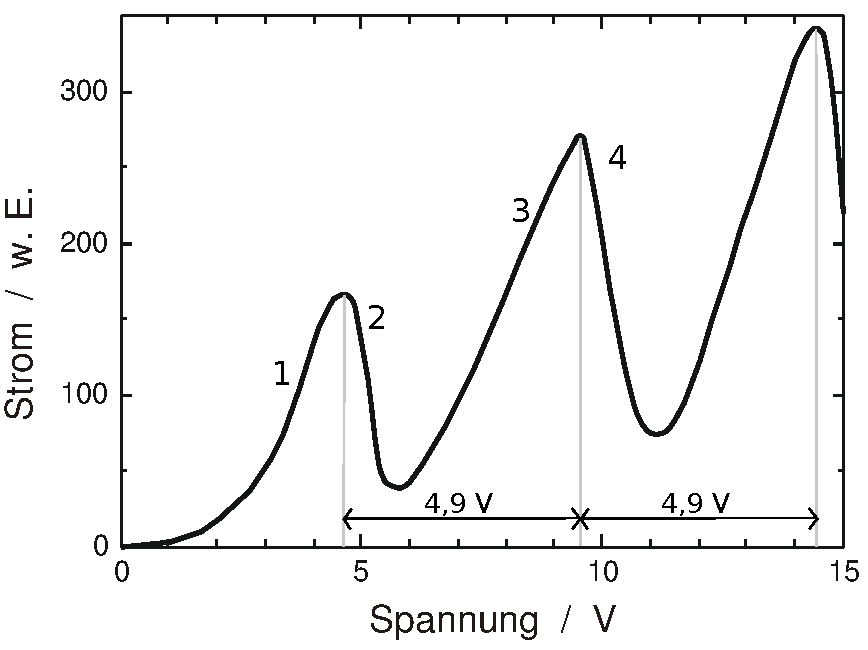
\includegraphics[width=0.5\textwidth]{./figures/franck-hertz_ergebnis.pdf}
\caption{Anodenstrom beim Franck-Hertz-Versuch mit Quecksilber, aufgetragen gegen die Beschleunigungsspannung; nach Originaldaten von Franck und Hertz. Quelle: \url{http://upload.wikimedia.org/wikipedia/commons/5/50/Franck-Hertz_de.svg} (abgerufen am 14.11.2014)}
\label{fig:franck-hertz_ergebnis}
\end{figure}

Bei der Durchführung des Versuches stellte man fest, dass der Anodenstrom sich wie in Abbildung \ref{fig:franck-hertz_ergebnis} verhält.
Man sieht dabei, dass in Abständen von \SI{4.9}{\volt} (der Wert gilt nur für Quecksilber) der Strom stark einbricht und ab den Minima jeweils einer Diodencharakteristik folgt \cite{demtroeder3}.
Der Grund dafür ist, dass die Elektronen auf der Beschleunigungsstrecke inelastische Stöße mit den Quecksilberatomen ausführen und diese dadurch anregen.
Die dabei an das Quecksilber abgegebene Energie steht den Elektronen nicht mehr zur Verfügung, um die Anode zu erreichen, der Strom bricht ein. 
Der Abstand der Maxima entspricht dabei genau der Anregungsenergie der Quecksilberatome.
In diesem Versuch soll die Übergangsenergie der Resonanzlinien von Quecksilber bestimmt werden. (ist das gleich der Anregungsenergie?)

\subsubsection{Röhrenelektronik}

\begin{itemize}
\item Glühemission
\item Raumladung
\item Elektronenbewegung in Triodensystem
\end{itemize}

\subsubsection{Thermodynamik und Stoßprozesse}

\begin{itemize}
\item Gaskinetik
\item Zwei-Phasen-System
\item (in-)elastische Stöße
\item mittlere freie Weglänge
\item Stoßquerschnitt
\item Gegenfeldmethode
\end{itemize}

\subsubsection{Quecksilberatom}

\begin{itemize}
\item LS- / jj-Kopplung
\item Termschema
\item Auswahlregeln
\item Resonanzabsorption
\end{itemize}

\section{Versuchsdurchführung}

\subsection{Versuchsbeschreibung}

\subsection{Aufbau}

\subsubsection{Hinweis zu einem der Geräte oder whatever}

\section{Messdaten}

\section{Auswertung}

\section{Diskussion}

\section{Zusammenfassung}

% BIBLIOGRAPHIE

% Maximale Anzahl der Einträge in Klammer
% Zitieren mit \cite{lamport94}
\begin{thebibliography}{9}

% Beispiel
\bibitem{np_richardson}
 Nobelprize.org,
 \emph{"The Nobel Prize in Physics 1928"}.
 Nobel Media AB 2014. Web. 15\\
 (\url{http://www.nobelprize.org/nobel_prizes/physics/laureates/1928/richardson-lecture.pdf} abgerufen am 15.11.2014)
  
\bibitem{demtroeder3}
	Wolfgang Demtröder,
	\emph{Experimentalphysik 3}.
	Springer Verlag,
	3. Auflage
\end{thebibliography}

\newpage

% APPENDIX
\begin{appendix}

\end{appendix}

\end{document}
